\subsection{Explicación general del diseño}
\par El modelo presentado se basa en un sistema de simulación que es configurado con los siguientes subsistemas:
\begin{itemize}
  \item \textbf{Sistema de construcción}: es el encargado de crear y almacenar los planes de construcción de pozos de extracción, plantas procesadoras y tanques de almacenamiento. También almacena los catálogos de plantas procesadoras y tanques de almacenamiento y gestiona las conexiones entre pozos de excavación, tanques de almacenamiento y plantas procesadoras.
  \item \textbf{Sistema de ejecución de criterios}: se encarga de llevar a cabo la ejecución de cada criterio del sistema.
  \item \textbf{Sistema de gestión de excavadoras}: posee el catálogo de excavadoras y gestiona su alquiler. También almacena el estado de las excavadoras alquiladas.
  \item \textbf{Sistema de gestión de parcelas}: Es quien conoce al yacimiento y administra las parcelas utilizadas y libres.
  \item \textbf{Sistema de extracción y reinyección}: Es quien se encarga de crear los eventos de extracción y reinyección sobre los pozos y almacenarlos.
\end{itemize}

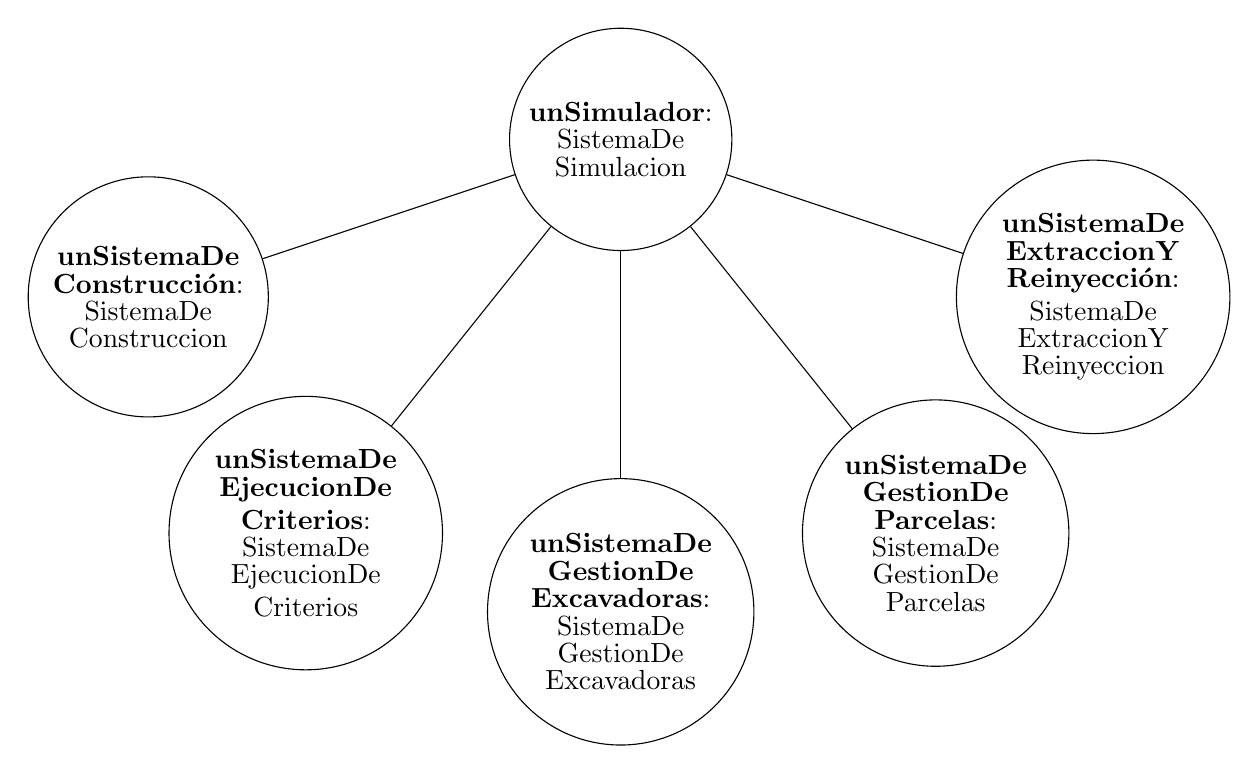
\begin{tikzpicture}
  \node[shape=circle,draw=black] (unSimulador) at (0,0) {\shortstack{\textbf{unSimulador}:\\SistemaDe\\Simulacion}};
  \node[shape=circle,draw=black] (unSistemaDeConstruccion) at (-6,-2) {\shortstack{\textbf{unSistemaDe}\\\textbf{Construcción}:\\SistemaDe\\Construccion}};
  \node[shape=circle,draw=black] (unSistemaDeEjecucionDeCriterios) at (-4,-5) {\shortstack{\textbf{unSistemaDe}\\\textbf{EjecucionDe}\\\textbf{Criterios}:\\SistemaDe\\EjecucionDe\\Criterios}};
  \node[shape=circle,draw=black] (unSistemaDeGestionDeExcavadoras) at (0,-6) {\shortstack{\textbf{unSistemaDe}\\\textbf{GestionDe}\\\textbf{Excavadoras}:\\SistemaDe\\GestionDe\\Excavadoras}};
  \node[shape=circle,draw=black] (unSistemaDeGestionDeParcelas) at (4,-5) {\shortstack{\textbf{unSistemaDe}\\\textbf{GestionDe}\\\textbf{Parcelas}:\\SistemaDe\\GestionDe\\Parcelas}};
  \node[shape=circle,draw=black] (unSistemaDeExtraccion) at (6,-2) {\shortstack{\textbf{unSistemaDe}\\\textbf{ExtraccionY}\\\textbf{Reinyección}:\\SistemaDe\\ExtraccionY\\Reinyeccion}};

  \path [-] (unSimulador) edge node[left] {} (unSistemaDeConstruccion);
  \path [-] (unSimulador) edge node[left] {} (unSistemaDeEjecucionDeCriterios);
  \path [-] (unSimulador) edge node[left] {} (unSistemaDeGestionDeExcavadoras);
  \path [-] (unSimulador) edge node[left] {} (unSistemaDeGestionDeParcelas);
  \path [-] (unSimulador) edge node[left] {} (unSistemaDeExtraccion);
\end{tikzpicture}
